%for reference to this section
\section{Einleitung}
\label{section:Introduction} 1350 Wörter

Einleitungstext......
wird nach Vollendung aller anderen Texte geschrieben, sowie Abstract und Kurzzusammenfassung.

\section{Hintergrund und Angriffsarten von XSS}
\label{section:History} 1350 Wörter

% genereller Überblick: was ist XXSS und welche Angriffsarten gibt es
Web Anwendungen sind ein fester Bestandteil, wenn es um online Dienste geht. Im selben Zuge werden aber immer mehr Anfälligkeiten in solchen entdeckt und offengelgt. Aber woher genau kommen diese Anfälligkeiten und wieso werden diese mit solche einer Vorsicht betrachtet, so \textcite{kirda2009}.

Laut \textcite[p.1]{mahmoud2017} ist eine Web Anwendung ein Programm, welches auf einem Server lauft und durch einen Web-Browser kundenseitig abgerufen wird.

\textcite[p.2]{hydara2015} melden, dass diese Sicherheitslücken erstmals in den 1990er, in den frühen Anfängen des World Wide Web, aufgetreten sind. Cross-Site-Scripting gehört zu den ernstzunehmendsten Schwächen wenn es um Web Anwendungen geht. Zu Schaden kommen dabei nicht nur der Source Code oder die Datenbank der Web Anwendung, sondern auch der Nutzer.

Nach \textcite[p.1]{mahmoud2017} ist einen Cross-Site-Scripting Attacke ein schadhafter JavaScript Code, welcher im Web-Browser des Opfers(Nutzer) ausgeführt wird um beispielsweise Zugangsdaten oder Kreditkarteninformationen des jeweiligen Nutzers zu stehlen.
Der Ablauf um einen solchen Code in die Anwendung injezieren zu können ist immer der Selbe, so \textcite{mahmoud2017}.
\begin{enumerate}
	\item Der Angreifer muss eine Schwachstelle in der Anwendung finden um seinen schadhaften Code in die Anwendung zu bringen und somit in weiterem Verlauf sensible Daten von seinem Opfer stehlen zu können.
	\item Das Opfer besucht die beschädigte Anwendung.
	\item Die Anwendung sendet eine Anfrage mit dem fehlerhaften Code im Body an einen Server.
	\item Wenn das Skript im Web-Browser des Opfers ausgeführt wird, kann der Angreifer diverse persönliche Informationen stehlen.
\end{enumerate}

\begin{figure}[ht]
	\centering
	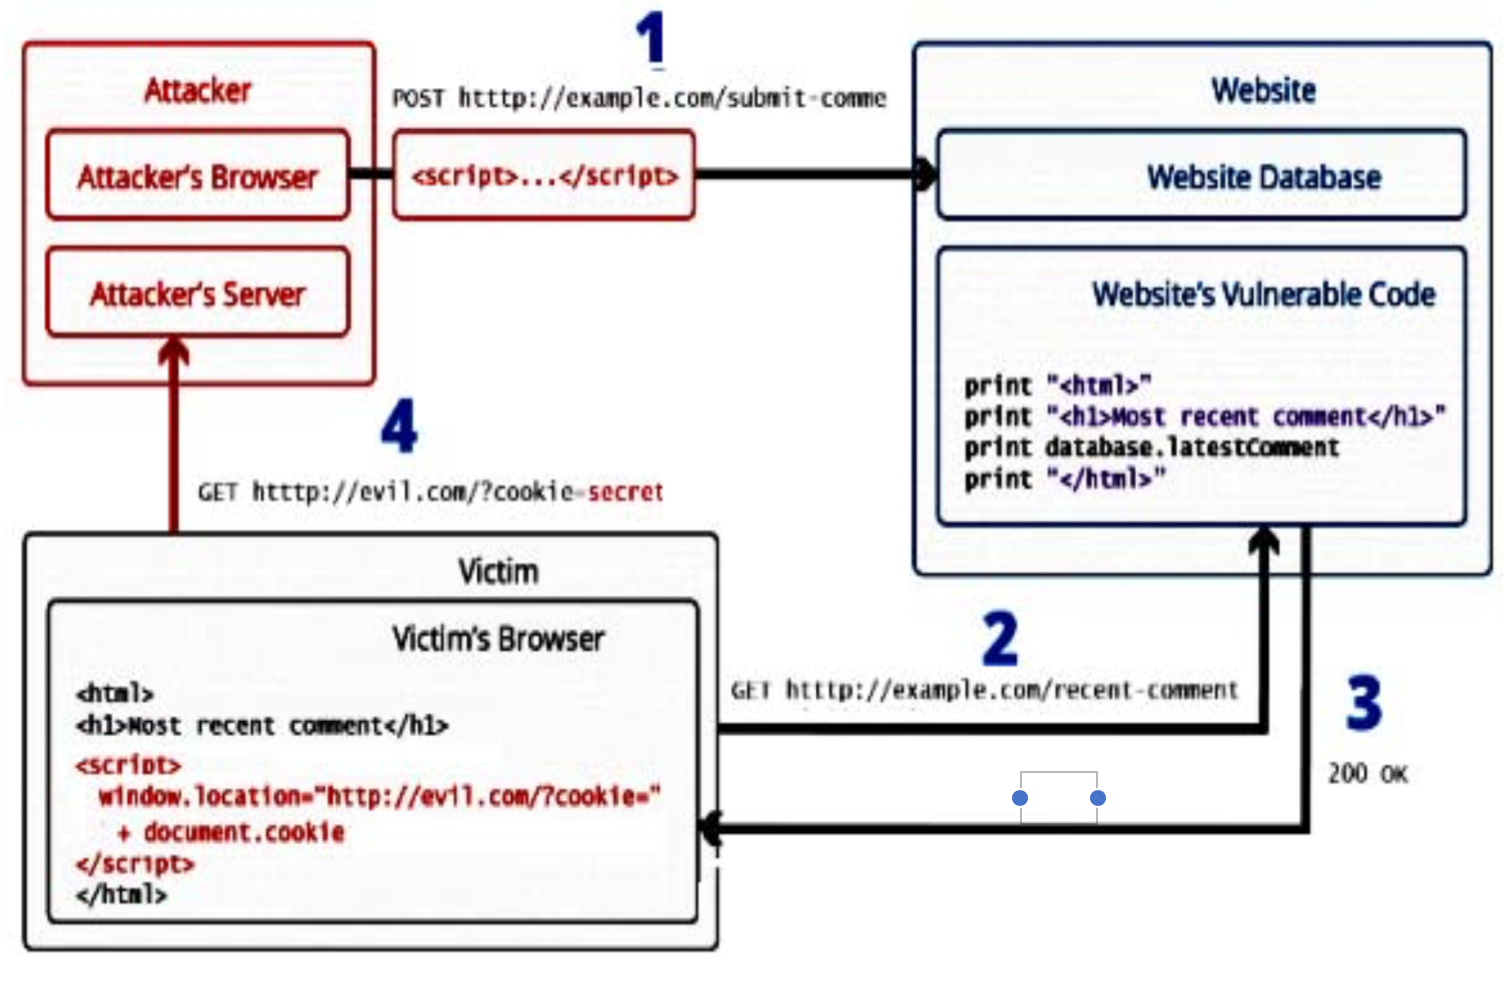
\includegraphics[width=0.75\linewidth]{images/XSS-attack-process.png}
	\caption{XSS Angriffsprozess}
\end{figure}



% Cross-Site-Scripting gibt es in vielen Ausführungen, \textbf{reflected, stored} and \textbf{DOM-based}

% Ab hier genauere Info über Angriffsarten
\subsection{DOM-basierte Attacken}
\label{subsection:DOM-based Attacks} 350 Wörter

Die DOM-basierte Attacken

\subsection{stored Attacken}
\label{subsection:stored attacks} 350 Wörter


\subsection{reflected Attacken}
\label{subsection:reflective attacks} 350 Wörter


% Neue Section
\section{Erkennunng}
\label{section:Detection} 1350 Wörter

Die Erkennung von Angriffen geht einher mit dessen Ausführung.

\subsection{Methode 1}
\label{subsection:Method1} 675 Wörter

\subsection{Methode 2}
\label{subsection:Method2} 675 Wörter

\section{Verhinderung} 1350 Wörter
\label{section:Prevention}

\subsection{Methode 1}
\label{subsection:Method1} 675 Wörter

\subsection{Methode 2}
\label{subsection:Method2} 675 Wörter
